\documentclass[a4j,12pt,]{jarticle}
 \usepackage[dvipdfmx]{graphicx}
 \usepackage{float}
 \usepackage{siunitx} %%SI単位系用
 \usepackage{amssymb, amsmath}
 \usepackage{ascmac,here,txfonts,txfonts}
\usepackage{listings,jlisting}
\usepackage[dvipdfmx]{color}
\lstset{%
  language={Python},
  basicstyle={\small},%
  identifierstyle={\small},%
  commentstyle={\small\itshape\color[rgb]{0,0.5,0}},%
  keywordstyle={\small\bfseries\color[rgb]{0,0,1}},%
  ndkeywordstyle={\small},%
  stringstyle={\small\ttfamily\color[rgb]{1,0,1}},
  frame={tb},
  breaklines=true,
  columns=[l]{fullflexible},%
  numbers=left,%
  xrightmargin=0zw,%
  xleftmargin=3zw,%
  numberstyle={\scriptsize},%
  stepnumber=1,
  numbersep=1zw,%
  lineskip=-0.5ex%
}
\begin{document}

{\noindent\small 第1回報告書 \hfill\today}
\begin{center}
  {\Large Kibanaを使用したElasticサーバーの確認}
\end{center}
\begin{flushright}
  祖父江匠真 \\
\end{flushright}

\section{はじめに}
MongoDB内, およびファイルサーバ内に保存された太陽光発電の環境データをElasticsearchサーバーに移行するプログラムを開発するにあたり, 現在Elasticsearchサーバーに保存されているJSONデータの構造を確認する必要があるので, Kibanaを使用して確認した.

\section{Kibanaへのアクセスとデータ確認}
引き継ぎ書 \cite{1}に記載されていたアドレスを使用して, Kibanaサーバーにアクセスした.
図\ref{p1}に, Elasticsearchサーバーに保存している太陽光発電の環境データのDocumentを示す.

\begin{figure}[H]
  \begin{center}
    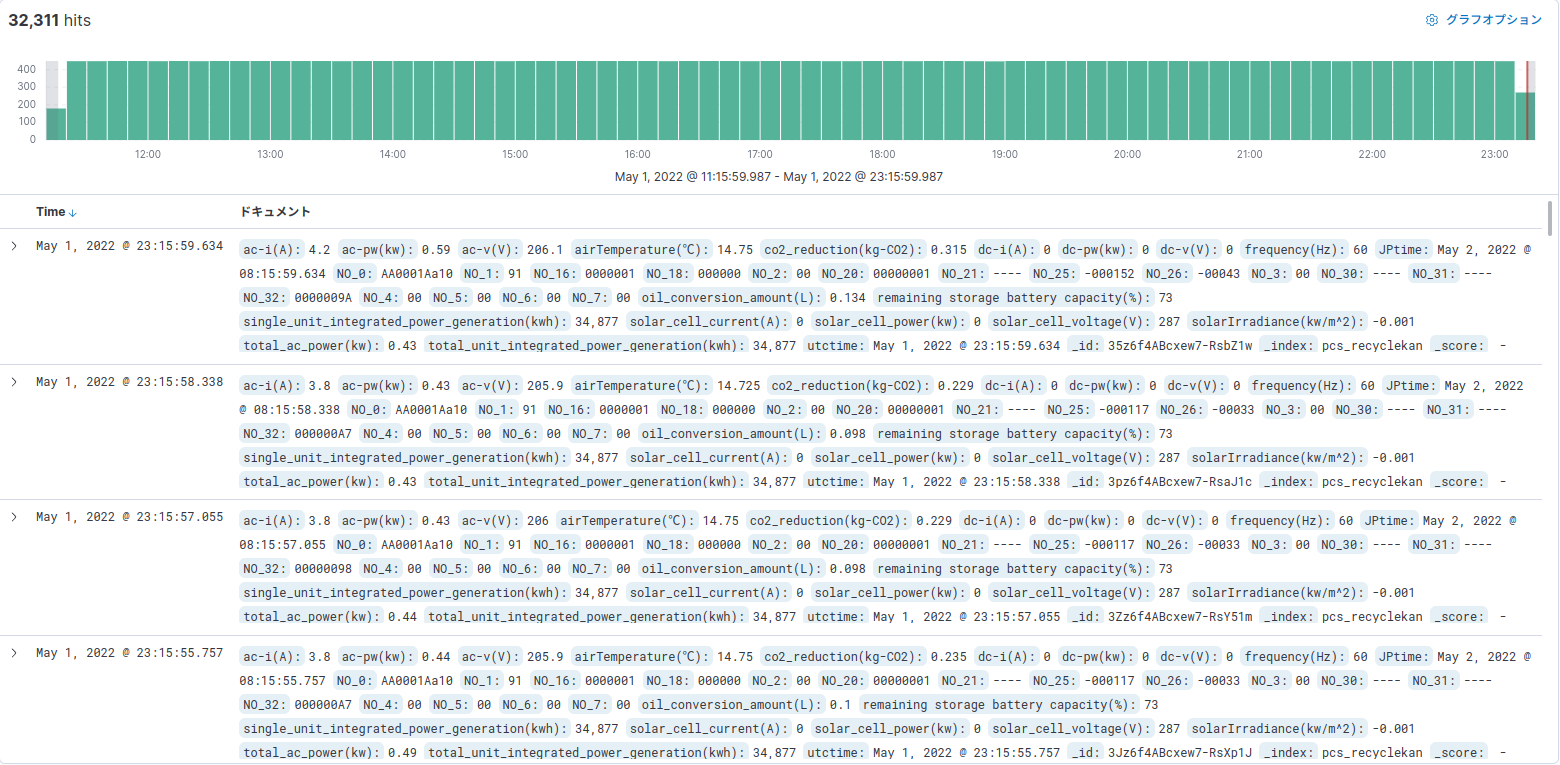
\includegraphics[width=160mm]{json.png}
    \caption{太陽光発電の環境データのDocument}
    \label{p1}
  \end{center}
\end{figure}

図\ref{p2}に図\ref{p1}のDocumentをJSON形式にしたものを示しているが, JSONデータのNO\_から始まるキーはRS485から送信された電文データをカンマごとに分割したものであり, Kibanaを使用した可視化システムの構築には不要なデータである.

\begin{figure}[H]
  \begin{center}
    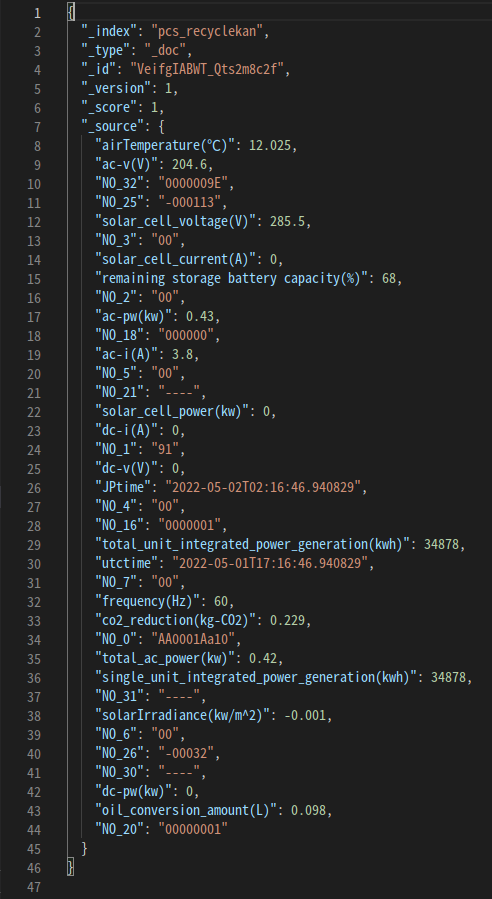
\includegraphics[width=130mm]{one_json.png}
    \caption{太陽光発電の環境データのDocumentをJSON形式にしたもの}
    \label{p2}
  \end{center}
\end{figure}

次に, このJSONデータを元にKibanaによって生成されたグラフを図\ref{p3}に示す.
また, 図\ref{p3}のグラフでは, JSONデータのsolarIrradiance(\si{\kilo\watt}/\si{\metre\squared}), airTemperature(\si{\degreeCelsius}), dc-pw(\si{\kilo\watt})キーの値を使用してグラフを生成している.

\begin{figure}[H]
  \begin{center}
    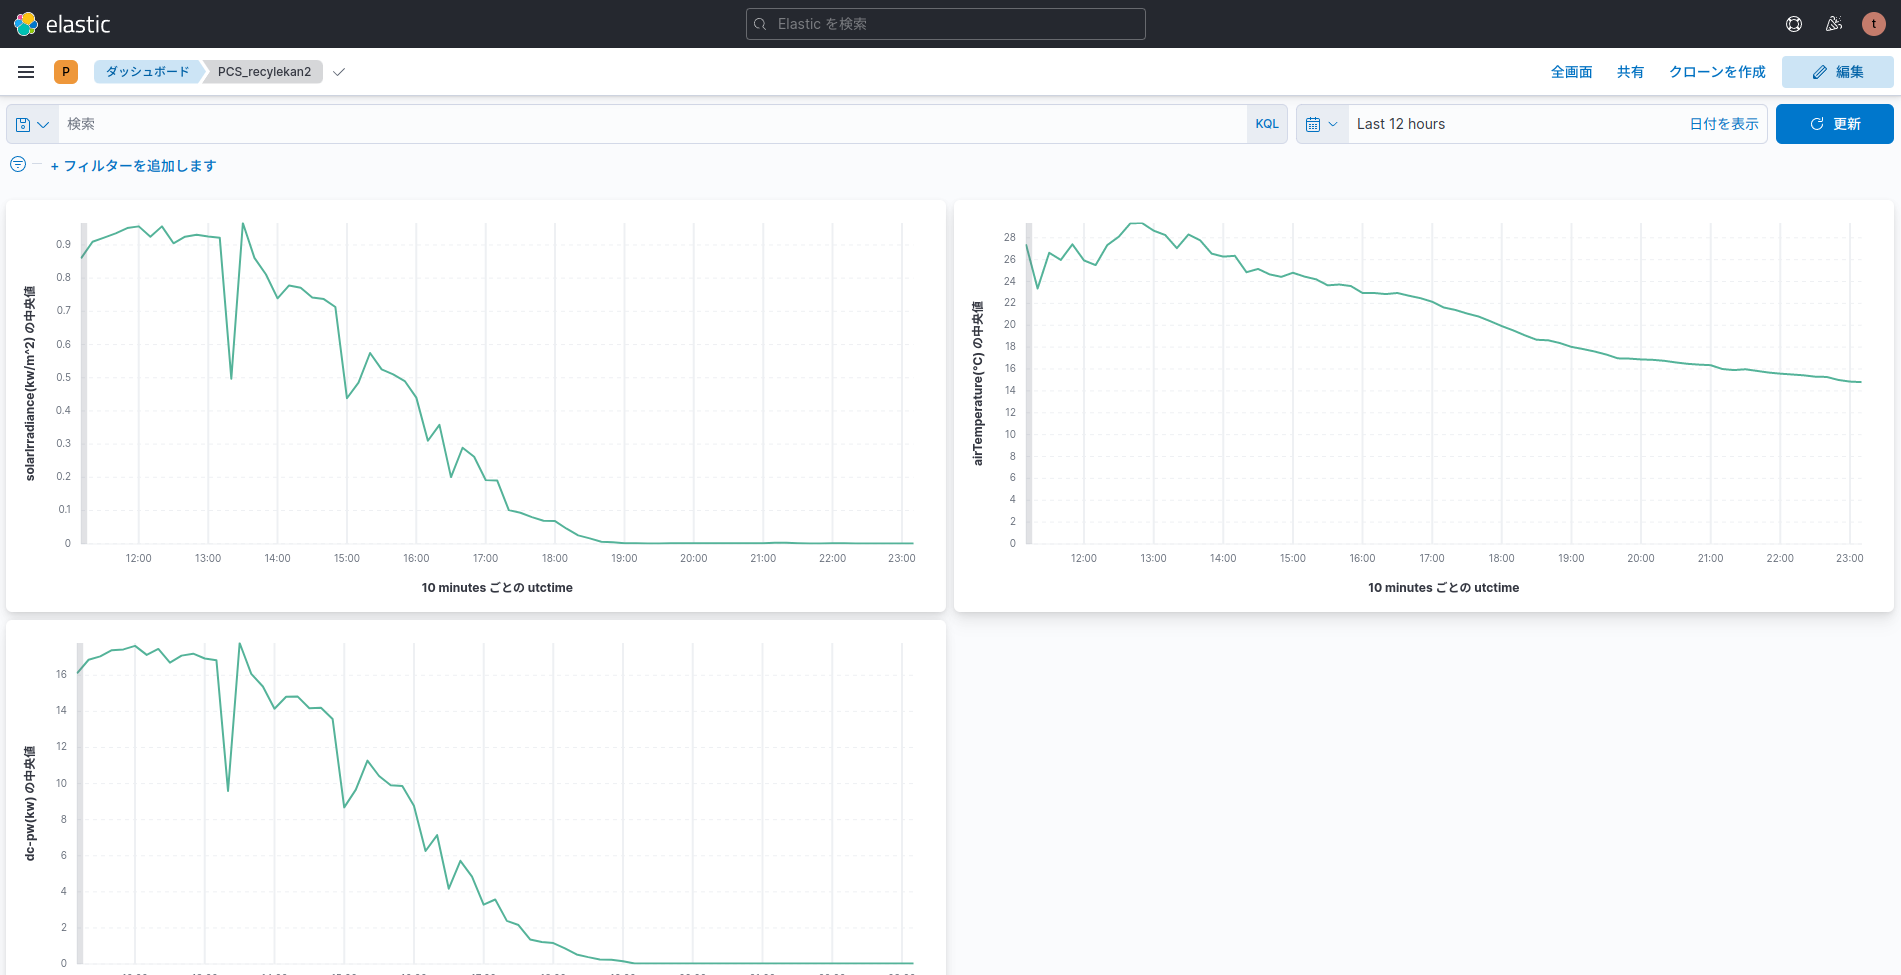
\includegraphics[width=160mm]{graph.png}
    \caption{Kibanaによって生成されたグラフ}
    \label{p3}
  \end{center}
\end{figure}

\section{おわりに}
今回は, Elasticsearchサーバーに保存されているデータをKibanaを使用して確認した.

\begin{thebibliography}{5}
  \bibitem{1}竹中駿介,”引き継ぎ書.pdf”, teams内,参照 May 1,2022.
\end{thebibliography}

\end{document}